This chapter presents a novel metaphor  to support coverage based debugging
visualization. It also provides details on  the realization of the metaphor, as
well as on the mechanisms made available to aid developers to narrow their
search for faults down to the most suspicious elements (class, method, and node)
of the system under analysis.

\section{Metaphor}\label{sec:metaphor}
The CodeForest metaphor is composed of three elements. Every class is
represented as a cactus. A branch is drawn in the cactus for every method within
a class. Thorns are associated with nodes. We represent nodes instead of
statements (or lines of code) because all statements of a node have the same
suspiciousness value since they are executed in sequencial order.

The positioning, coloring, sizing and the thickness of the forest's cacti are
determined  by their suspiciousness values. First, the cactus having the lowest
suspiciousness rank is placed in the upper left corner of the terrain.
Then, the element having the second lowest rank is placed to the right side of
the previous cactus, and so on. When there is no more space available at the
current row, the cactus to be inserted is placed in the left corner just below
the previous row. This process goes on until there is no more cacti to be placed
in the terrain.

Figure~\ref{fig:codeforestmetaphor} illustrates this rationale with the lowest
ranked cactus  painted in green on the upper left corner; a middle-ranked cactus
painted in yellow  positioned in the middle; and the highest ranked cactus
painted in red placed in the lower right corner---the inspiration for this
grid-layout comes from Figure~\ref{fig:tufte1983visual}, available in
\cite{tufte1983visual}[p. 108].
The intuition being that these are the system's most likely classes in which the
defect might be found.
In addition, in order to decrease the developer's distraction levels to a
minimum, the higher the rank, the thicker and taller the cactus is. By doing so,
the intent is to give as much as possible attention to the first rows where the
highest ranked cacti are located.
The mapping between color and suspiciousness also applies to thorns whose colors
varies from red (representing the highest ranked node) to green (representing
the lowest ranked node).

\begin{figure*}
    \centering
    \subfigure[CodeForest] {
        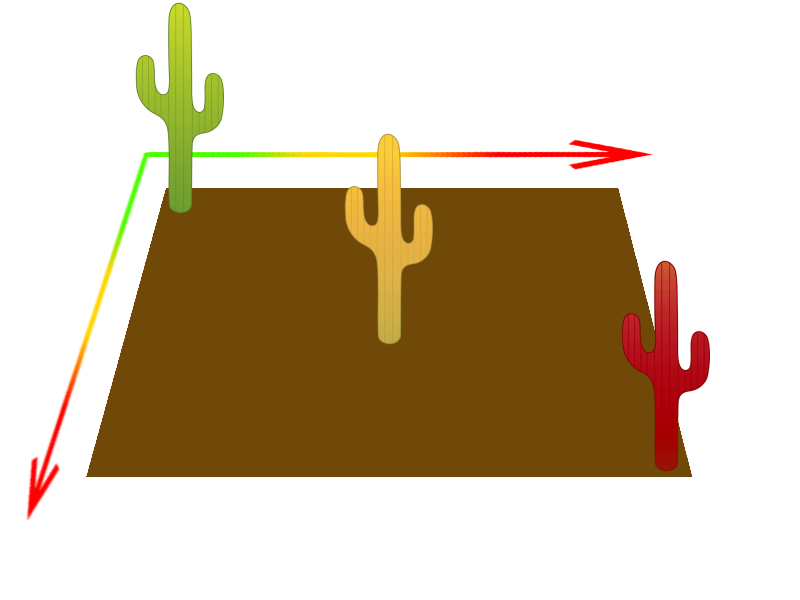
\includegraphics[width=\linewidth]{figures/metaphor}
        \label{fig:codeforestmetaphor}
    }
    \subfigure[Cactus] {
        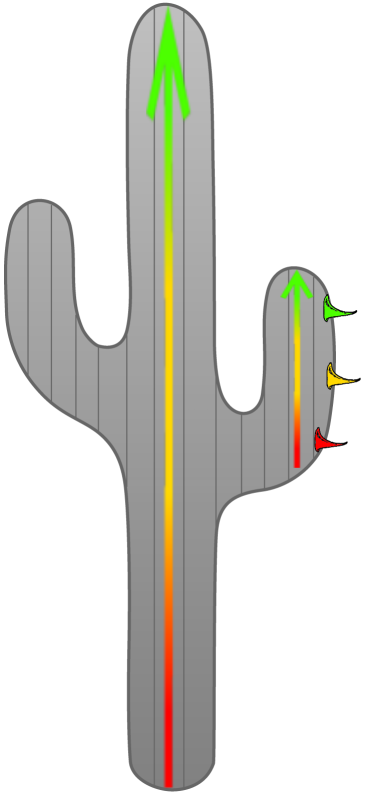
\includegraphics[width=.30\linewidth]{figures/internal_metaphor}
        \label{fig:cactusmetaphor}
    }
    \caption{Proposed metaphors}
\end{figure*}

\begin{figure*}
  \centering
    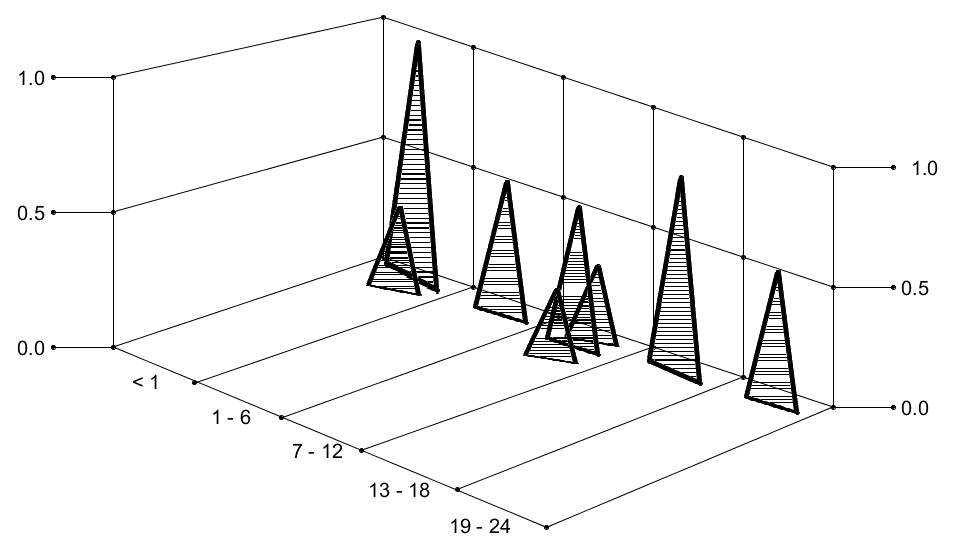
\includegraphics[width=\linewidth]{figures/tufte1983visual}
  \caption{Interpretation of Tufte's serial echocardiographic assessments of the severity of
  regurgitation in the pulmonary autograft in patients~\cite{tufte1983visual}}
  \label{fig:tufte1983visual}
\end{figure*}

This rationale is not applied to branches since painting them with  colors
different from the color (ranking) of the cactus might confuse the developer.
Therefore, in order to keep the metaphor informative without turning it into a
gathering of colors, a second mapping  adds ``weight" to a branch. Thus, the
highest ranked branches would have a greater weight than lowest ranked branches,
with the former positioned closer to the ground, in opposition to the latter.
Figure~\ref{fig:cactusmetaphor} illustrates the rationale applied for both
thorns and branches regarding their positioning.

The next section describes the realization of the metaphor by presenting in
details the strategies employed to achieve the objectives described in
Chapter~\ref{ch:introduction}.

\section{Metaphor realization}

In the previous section,  CodeForest's underlying intuition was presented. In
this section, we present how coverage debugging information associated with
classes, methods, and nodes is mapped into a visual representation of a forest
of cacti.  The  forest elements  positioning, coloring, and sizing  and their
relation to suspiciousness are described next.

\subsection{Positioning the elements}

The forest is internally represented as a grid where the position of a cactus is
determined by its CH suspiciousness value. The first task is to determine the
width of the terrain in which the cacti will be positioned.
Algorithm~\ref{alg:terraindim} demonstrates the steps taken to calculate the
ideal width. Briefly, the algorithm calculates the linear width occupied by a
cactus by looking for the widest branch on each size
(\textit{maxLeftBranchWidth} and \textit{maxRightBranchWidth} functions). Next,
the number of cacti plus one is multiplied by the largest trunk radius found
(\textit{findMaxRadius} function).
The obtained value is added to the summation of the branch size. The ideal
terrain width is the result of the division between the sum of all previous
values and the square root of the number of cacti in the forest.

As soon as the terrain's width is defined,  the cacti's positioning, detailed in
Algorithm~\ref{alg:positioning}, follows. Cacti are added to a row until the
current row gets full (lines 6 to 8), i.e., adding another cactus would cause it
to ``fall off" the terrain. When this situation happens, the current cactus is
promoted to a newly created row. This algorithm goes on until there are no more
cacti to be added. Then, the free space of every row is divided equally among
cacti. Thus, when a single cactus occupies an entire row, it is located right in
the middle of it, instead of being positioned in the rightmost position. This
particular situation can be observed in the aerial view of the Ant\footnote{Ant
is the Apache project tool for building applications, especially Java
applications (\url{http://http://ant.apache.org/}).} program's forest presented
in Figure~\ref{fig:ant_wireframe_overview}. The cactus with the highest rank is
located right in the middle of the front row. It is also possible to notice how
cacti of different sizes and heights fill different portions of the terrain.

\begin{figure*}
  \centering
    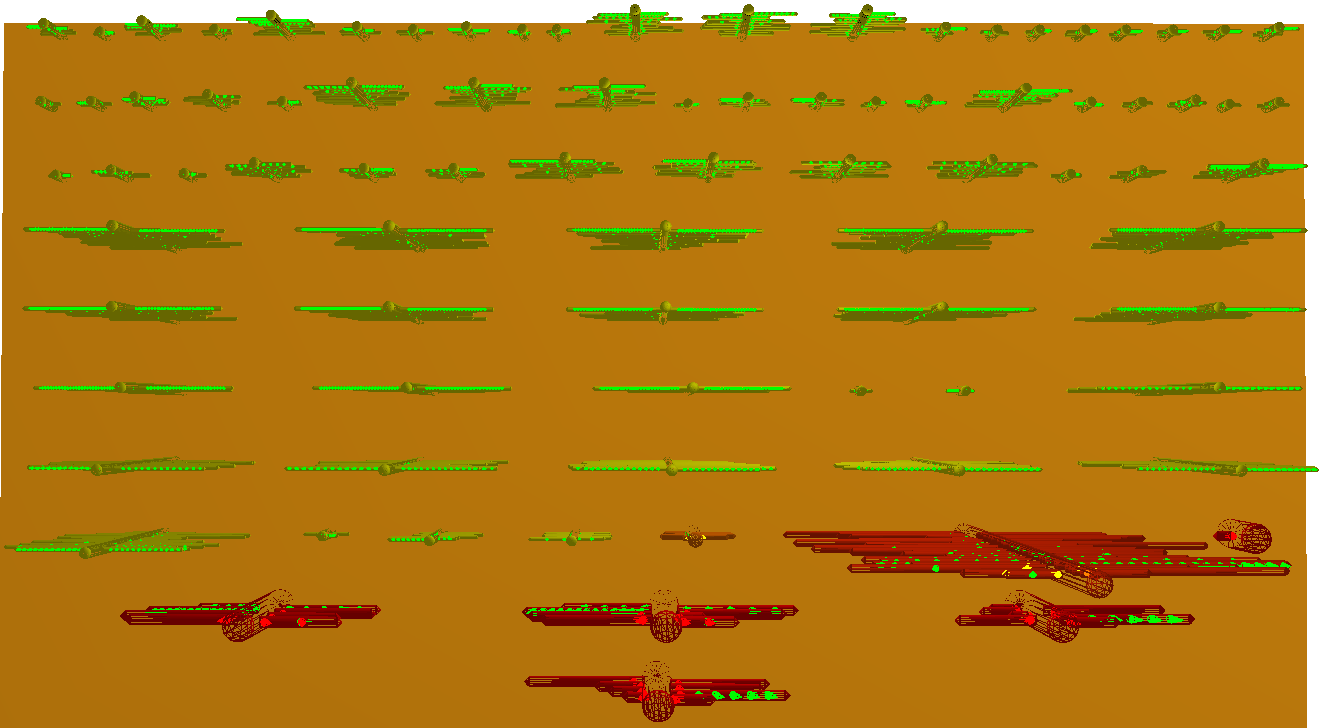
\includegraphics[width=\linewidth]{figures/ant_wireframe_overview}
  \caption{Aerial view of  Ant's forest of cacti (wireframe).}
  \label{fig:ant_wireframe_overview}
\end{figure*}

\begin{algorithm}[htbp]
\KwData{An ordered array of records containing CH data (\textit{susp},
\textit{number}) -- \textit{classDataList}}
\KwResult{Grid width dimension}
\BlankLine
\Begin {
    $sum \leftarrow 0$\;
    $count \leftarrow 0$\;
    $Cactus[\text{ }]$ $cacti$\;
    \ForEach{$classData$ \textbf{in} $classDataList$}
    {
        Cactus $cact$ $\leftarrow$ \textbf{new} Cactus($classData$)\;
        $sum \leftarrow sum + cact$.maxLeftBranchWidth $+$
        $cact$.maxRightBranchWidth\; $cacti[count] \leftarrow cact$\; $count \leftarrow count + 1$
    }
    $sum \leftarrow sum + ((count + 1) * findMaxRadius(cacti))$\;
    \Return $sum / \sqrt{count}$;
}
\caption{Ideal grid width calculation}
\label{alg:terraindim}
\end{algorithm}

\begin{algorithm}[htbp]
\KwData{An ordered array of cactusData -- \textit{cactiList}, ideal grid width -- \textit{width}}
\KwResult{Each cactus gets its position on the grid}
\BlankLine
\Begin {
    $i \leftarrow 0$\;
    $grid$ $\leftarrow$ \textbf{new} $Grid$()\;
    $grid$.row[$i$] $\leftarrow$ \textbf{new} $Row$()\; 
    \ForEach{$cactusData$ \textbf{in} $cactiList$}
    {
        $gap \leftarrow width - grid$.row[$i$].currentWidth\;
        \If {($cactusData$.width $\leq gap$)}{
            $grid$.row[$i$].add($cactusData$)\;
        } \Else {
            $i \leftarrow i + 1$\;
            $grid$.row[$i$] $\leftarrow$ \textbf{new} $Row$()\;
            $grid$.row[$i$].add($cactusData$)\;
        }
        $grid$.row[$i$].currentWidth $\leftarrow$ $grid$.row[$i$].currentWidth
        $+$ $cactusData$.width\; }
}
\caption{Cactus positioning}
\label{alg:positioning}
\end{algorithm}

Cacti are positioned in each row according to the description provided in
Section~\ref{sec:metaphor}. Each row is populated from the back to the front
(lowest to the highest rank); in a row, cacti are ordered from from right to
left (highest to the lowest rank). The goal is to focus the programer's
attention onto the first rows where the highest ranked cacti are positioned.
Thus, these are the classes most likely to contain faults.
Figure~\ref{fig:xml-security-metaphor} shows the
XML-security\footnote{XML-security  is a component library implementing XML
signature and encryption standards, supplied by the XML subproject of the open
source Apache project (\url{http://santuario.apache.org/}).} program represented
as a forest of cacti. In this figure, the most suspicious class is the one up
front at far right, indicated by the blue circle.

Since the position of the elements in the scene plays a crucial function in
capturing the programer's attention, our strategy is to add ``weight'' to the
most suspicious branches, making them closer to the trunk's base. Let us say
that the defect is not present in the most suspicious class in
Figure~\ref{fig:xml-security-metaphor}. The next cactus to be analyzed is at the
very  left of the most suspicious class in the same row. The first  branch to be
scrutinized is the one closest to the base as indicated by the yellow circle in
the figure.

\begin{figure*}
  \centering
    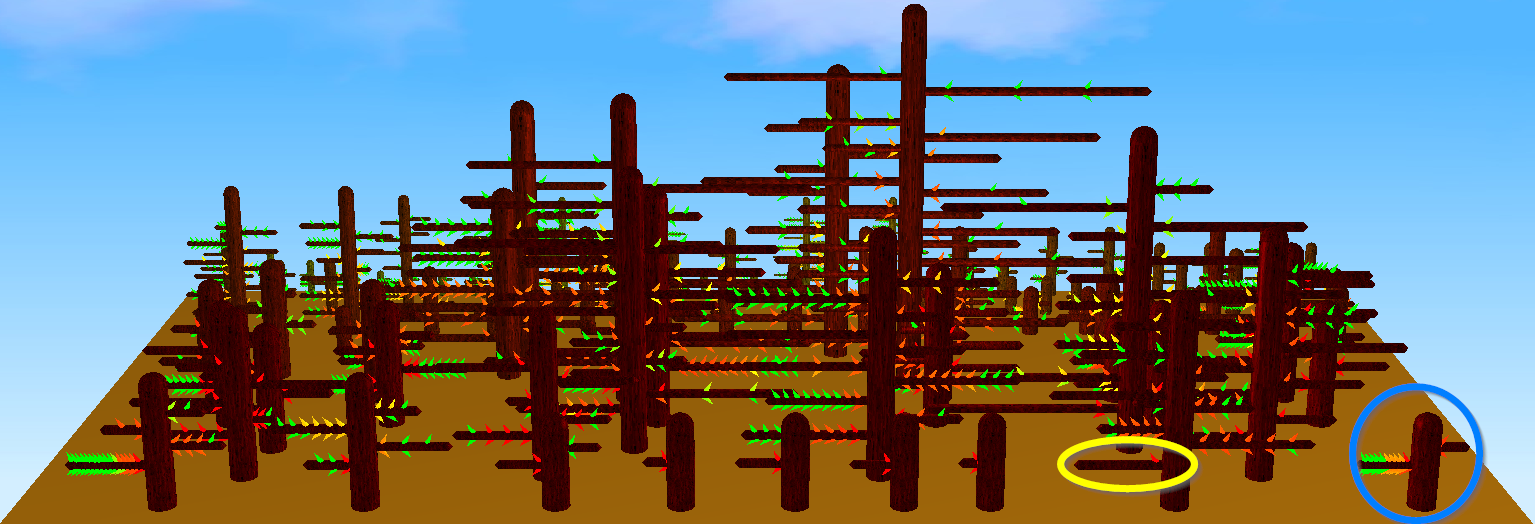
\includegraphics[width=\linewidth]{figures/xml-security-metaphor.png}
  \caption{The XML-security program represented as a forest of cacti.}
  \label{fig:xml-security-metaphor}
\end{figure*}

Unlike other strategies based on tree metaphors~\cite{erra2012towards},
CodeForest branches are always in a parallel position, never facing the
developer. By doing so, a bigger number of thorns are shown without the need to
rotate or translate the scene.

Nodes, represented by thorns, are alternately positioned on a branch. Starting
from the trunk, the first thorn is rendered with the tip pointing upwards. The
same exact position holds the second thorn, with its tip pointing downwards. The
process continues until all thorns are rendered.

Thorns are positioned taking into account their suspiciousness value determined
by a ranking heuristic.  The more suspicious a node, the  closer  its
corresponding thorn will be to the trunk. The thorn with the upward tip is more
suspicious than another parallel thorn with a downward tip. Interestingly, there
is no relationship between the position of a node in the method and its position
in the branch. Two ``distant'' nodes in the code can be close in the branch
depending on their suspiciousness values.

The most suspicious class in Figure~\ref{fig:xml-security-metaphor} has two
branches, being the most suspicious node the red one closes to the trunk in the
lowest branch with the upward tip.

\subsection{Coloring the elements}
\label{subsec:coloring}
The elements' coloring is determined by their suspiciousness rank.  All
suspiciousness values are in the interval $[0,1]$, where $0$ is the lowest
suspicious value and $1$ is the highest one. As a defect is ultimately caused by
one or more lines of code (or the absence of it), CodeForest highlights the
thorns (the abstraction for lines of code) in the scene by utilizing the same
color pattern proposed by Jones et al. \cite{jones2002visualization}.

The pure green color represents the lowest rank (0). Analogously, the pure red
color is associated with the highest ranked elements (1). The intermediate value
is yellow and, as the rank moves from $1$ to $0.5$, the color goes from red to
orange and finally pure yellow. When it reaches the lower half, the color varies
from pure yellow to pure green.

The coloring of trunks occurs in the same way as thorns. Except that shades used
in this operation are darker, both for red and green. Our motivation, as
previously stated, is to draw the developer' attention to thorns since cacti and
branches are highlighted, especially, by their positioning.

\subsection{Sizing the elements}
The calculation of the height of a trunk takes two class-related properties into
consideration: the CH suspiciousness value and the number of methods belonging
to it. An alternative approach would be to only take the latter into consideration,
which could lead to distractions when using it. This would happen in the
presence of a class with a large number of methods (for instance, more than
thirty) and a low CH suspiciousness value. One example of such situation is the
classic Java container class: it has no behavior -- just attributes -- with a
getter and setter method for each attribute. Such a big cactus, even when
located in the back of the forest, is able to draw the user's attention to it,
yet with minimal chances of containing a defect.

One possible solution would have been to just display cacti with higher chances
of containing the defect, leaving harmless classes out of the forest. Although
it solves the stated problem, it also creates another one by imposing an
obstacle to visualizing the software as a whole. In order to preserve the
``whole-system-as-a-cacti-forest'' feature offered by CodeForest, we decided
that a better strategy would be to change the sizing of elements, based on the
suspiciousness value.

Before getting into the details of our solution, we first offer an explanation
of how a cactus is build. CodeForest utilizes three building blocks to construct
a cactus: cylinders (Figure~\ref{fig:cylinder}), spheres
(Figure~\ref{fig:sphere}) and cones (Figure~\ref{fig:cone}).
Every cactus in a forest is made from the same unit of construction, a
fictitious cylinder with radius $R$ e height $H$, capable of holding two
branches each.
The final height of a trunk can be calculated by the equation: $TrunkHeight = (H
* (\frac{M}{2})) + H$, where $M$ denotes the number of methods of a class and
the extra $H$ refers to the base cylinder, which holds no branches. This process
results in a central single-piece cylinder, aligned with the $y$ axis, with a
semi-sphere lying at its top (Figure~\ref{fig:wireframe}).

\begin{figure*}
    \centering
    \subfigure[Cylinder] {
        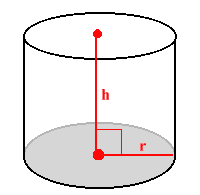
\includegraphics[width=.30\linewidth]{figures/cylinder}
        \label{fig:cylinder}
    }
    \subfigure[Sphere] {
        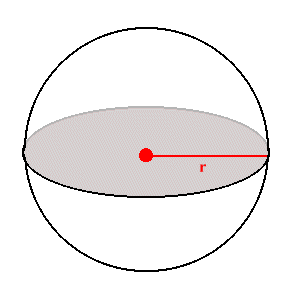
\includegraphics[width=.30\linewidth]{figures/sphere}
        \label{fig:sphere}
    }
    \subfigure[Cone] {
        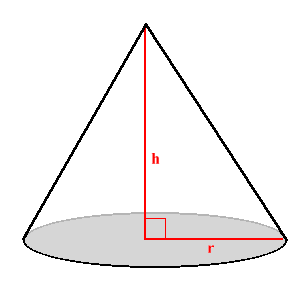
\includegraphics[width=.30\linewidth]{figures/cone}
        \label{fig:cone}
    }
    \caption{CodeForest primitives}
\end{figure*}

A branch is made of a single cylinder, aligned with the $x$ axis with a cone as
its tip. The radius value used to define the branch is derived from the value of
$R$. The width of the branch, on the other hand, is randomly picked among
several candidates with slightly small variations, where the shortest one is the
branch with no free space among thorns and the biggest one is at most two
thirds the size of the trunk. Finally, thorns are cones with a fixed radius,
also derived from $R$.

To avoid the problem of huge harmless cacti, we decided to establish the size of
the cacti (i.e., the classes) based on their CH suspiciousness value.
To accomplish this task, we defined a taxonomy comprised of four categories,
presented in Table~\ref{tab:sizing}.
Then, the minimum values of $H$ and $R$ are determined. Finally, the
trunk-building phase was adjusted to give these values a boost, based on the
assigned category. As explained earlier, every dimension of every part of the
trunk is obtained from the values of $H$ and $R$. Thus, this strategy resulted
in a forest with cacti varying not only in color and position, but also in size
and thickness. Additionally, we also defined that each category would also
define a maximum size for a branch. Table~\ref{tab:sizing-example} contains
several examples of trunk dimensions (height, radius, and maximum branch size)
calculated from the CH suspiciousness value and the number of methods found
inside a class. 

\begin{table}[H]
\begin{center}
    \caption{Sizing strategy}
    \label{tab:sizing}
    \begin{tabular}{c c c c c}
        \shortstack{Category\\name} & \shortstack{Radius boost} &
        \shortstack{Height boost} & \shortstack{Max branch
        size\\(cactus height)}  & \shortstack{Suspiciousness\\value (CH)}\\ \hline\hline Extra
        small & 1.0$R$ & 1.0$H$ & 33\% &  CH $< .45$\\
        Small & 1.5$R$ & 1.5$H$ & 33\% &  $.45\leq$ CH $< .65$\\
        Normal & 2.0$R$ & 1.8$H$ & 33\% &  $.65\leq$ CH $< .85$\\
        Big & 3.0$R$ & 3.0$H$ & 66\% &  $.85\leq$ CH $\leq 1.00$ \\
        \hline
    \end{tabular}
\end{center}
\end{table}


\begin{table}[H]
    \begin{center}
    \caption{Sizing example}
    \label{tab:sizing-example}
    \begin{tabular}{c c c c c c}
        \shortstack{CH} & \shortstack{Category} &
        \shortstack{Methods} & \shortstack{Height} &
        \shortstack{Boosted\\height} & \shortstack{Max\\branch size}\\
        \hline \hline
        0 & Extra small & 10 & 6$H$ ($\lceil\frac{10}{2}\rceil+1$) &
        6$H$ ($6*1$) & 2$H$ ($6*\frac{1}{3}$)\\
        .56 & Small & 5 & 4$H$ ($\lceil\frac{5}{2}\rceil+1$) & 6$H$
        ($4*1.5$) & 2$H$ ($6*\frac{1}{3}$)\\
        .68 & Normal & 20 & 11$H$ ($\lceil\frac{20}{2}\rceil+1$) &
        19.8$H$ ($11*1.8$) & 6.6$H$ ($19.8*\frac{1}{3}$)\\
        .89 & Big & 3 & 3$H$ ($\lceil\frac{3}{2}\rceil+1$) & 9$H$ ($3*3$)
        & 6$H$ ($9*\frac{2}{3}$)\\
        \hline
    \end{tabular}
    \end{center}
\end{table}

If we take the second line of Table~\ref{tab:sizing-example}, we can see a class
which has a CH score of 0.56. According to Table~\ref{tab:sizing}, this class
will be mapped into a \textbf{small} cactus. Because it contains five methods,
it will require three cylinders (one for each pair of methods) and one for the
base, which gives a calculated height of four $H$. But, this category receives a
small boost in its height (50\% in this case), resulting in a final height of 6
$H$ (each cylinder will be 1.50 $H$ high). If we look at Table~\ref{tab:sizing}
again, the maximum branch size must be, at most, 33\% of the final height, which
gives a maximum length of 2 $H$ for each branch.

Figure~\ref{fig:wireframe} shows the basic layout of a cactus classified as
``Big''. After the wireframe rendering stage takes place, the Java3D framework
then applies the bark texture on the structure.

\begin{figure*}
  \centering
    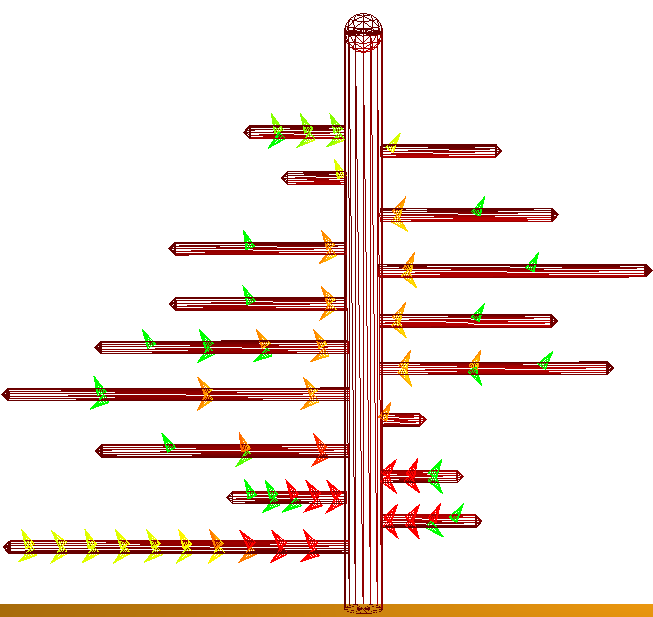
\includegraphics[width=\linewidth]{figures/wireframe}
  \caption{Wireframe of a cactus and its elements.}
  \label{fig:wireframe}
\end{figure*}

\section{CodeForest prototype}

\label{sec:prototype}
 
We developed a prototype implementing the CodeForest metaphor to evaluate its
usefulness in supporting coverage based debugging. The strategies to position,
color, and size the elements of the forest were implemented as well as
operations allowing the developer to manipulate these elements  to narrow down
the fault site. In what follows, we describe the prototype's operations.


\subsection{Basic resources}

Figure~\ref{fig:xml-security-codeforest} shows the XML-security program being
visualized using the CodeForest prototype.
The screen is divided in three main working areas as indicated by numbers 1, 2
and 3 in the figure. Area 1 occupies the largest space in the screen and is
where the forest of cacti is presented.  It is also in area 1 where the
developer carries out basic manipulation actions available on every 3D
prototype, namely, translation, rotation, and zooming.

The source code is available at anytime during the fault localization process.
If the developer wants to inspect it, she can click on any element of the scene.
If a cactus is clicked the first line of the class is displayed in a text area
under the forest (area 2). Similarly, the first line of a  method is presented
when the associated branch is clicked.
Finally, if a thorn  is clicked, the interface displays the lines of code of its
associated node highlighted accordingly to the node's suspiciousness.

\begin{figure*}
  \centering
    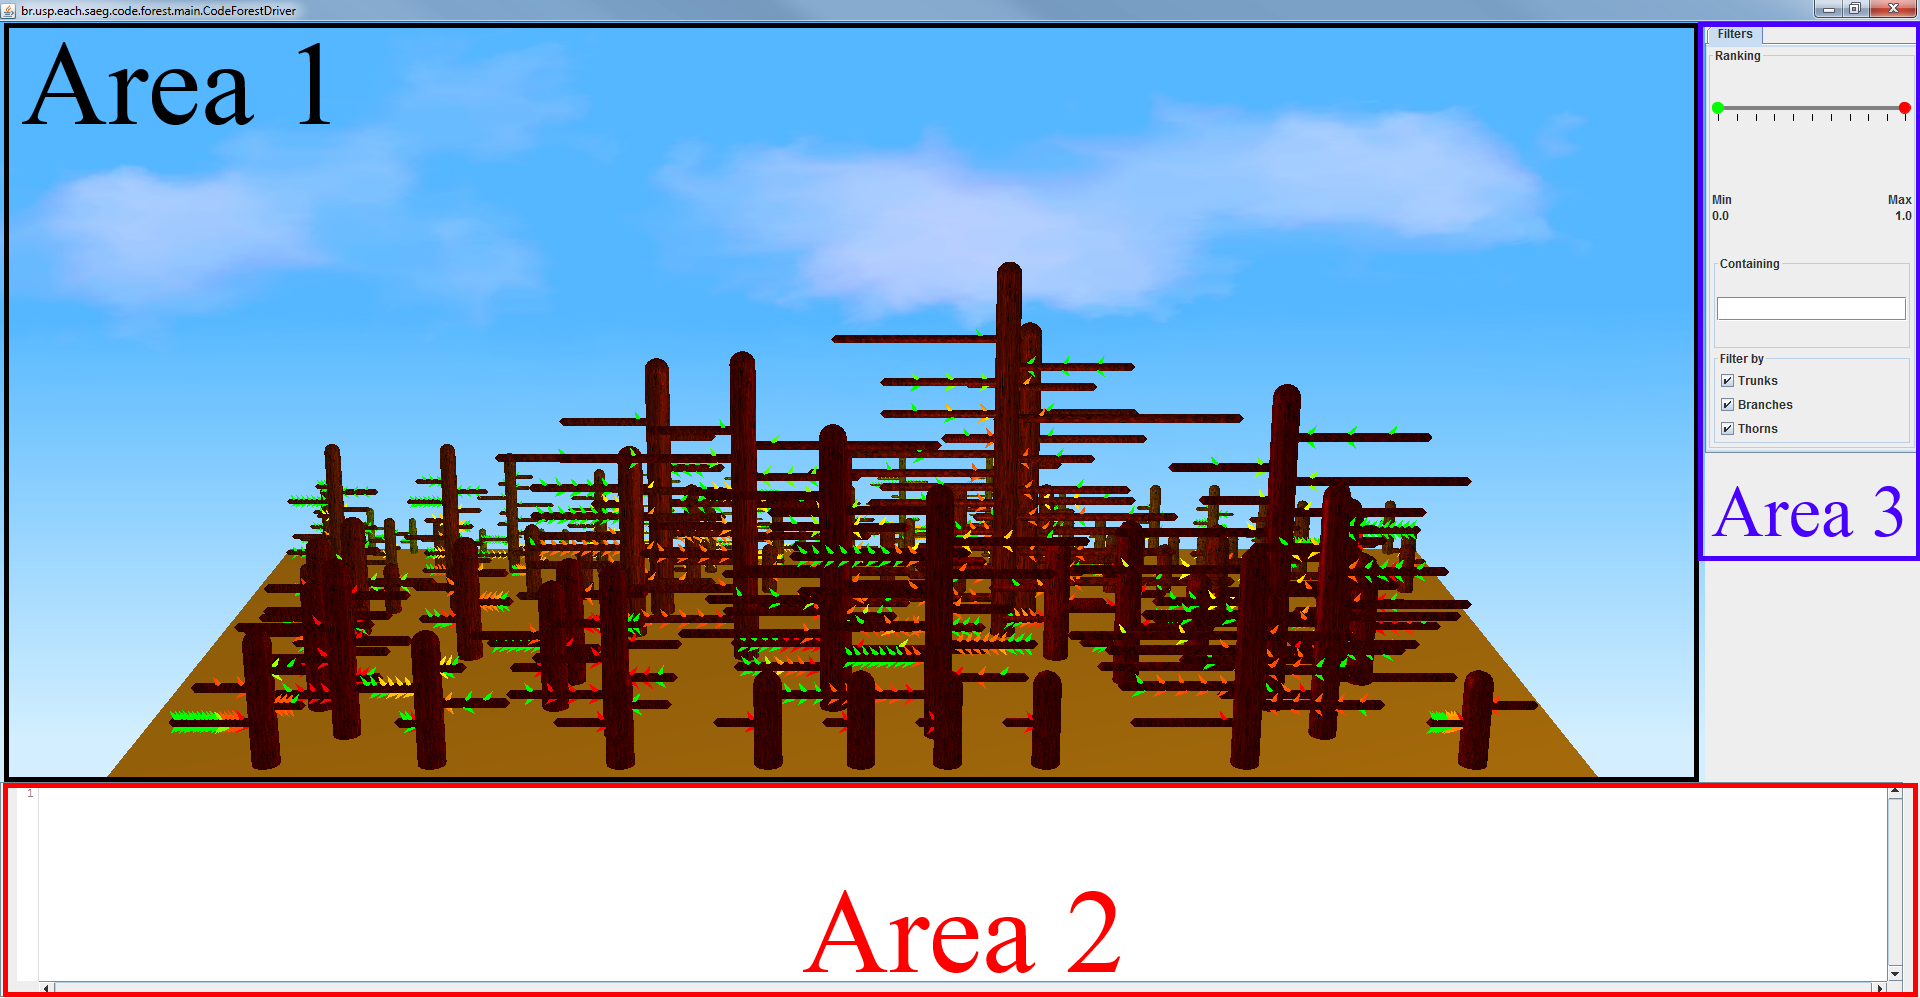
\includegraphics[width=\linewidth]{figures/xml-security-codeforest.png}
  \caption{The XML-security program visulized with the CodeForest prototype.}
  \label{fig:xml-security-codeforest}
\end{figure*}

\subsection{Trimming and filtering operations}

In Figure~\ref{fig:xml-security-codeforest}, one can observe that the forest of
cacti can be quite dense hampering the developer's ability to focus onto highly
suspicious thorns, branches, and cacti. Resources  to trim and filter elements
of the forest were implemented to enhance the developer's ability to localize
the fault.  These resources are inline with Parnin and Orso's suggestions to
leverage coverage based debugging~\cite{parnin2011automated}.

The trimming operation allow users to trim cacti, branches and thorns
simultaneously or one scene element at a time. The trimming operation is actived
when the developer defines both a lower bound and an upper bound of 
suspiciousness values using a slider available at the right upper corner of the
screen (area 3 of Figure~\ref{fig:xml-security-codeforest}).

The slider, which we call \textit{trimmer}, controls the suspiciousness  of the
elements to be presented. All elements whose suspiciousness value lies outside
these limits are removed from the forest.  The check box in area 3 allows the
developer to define which scene elements to be trimmed.  By positioning the
trimmer at the far right, she will  select scene elements with highest
suspiciousness value (1.0). As a result, the density of the forest is reduced as
shown in Figure~\ref{fig:xml-security-trimmed}.

\begin{figure*}
  \centering
    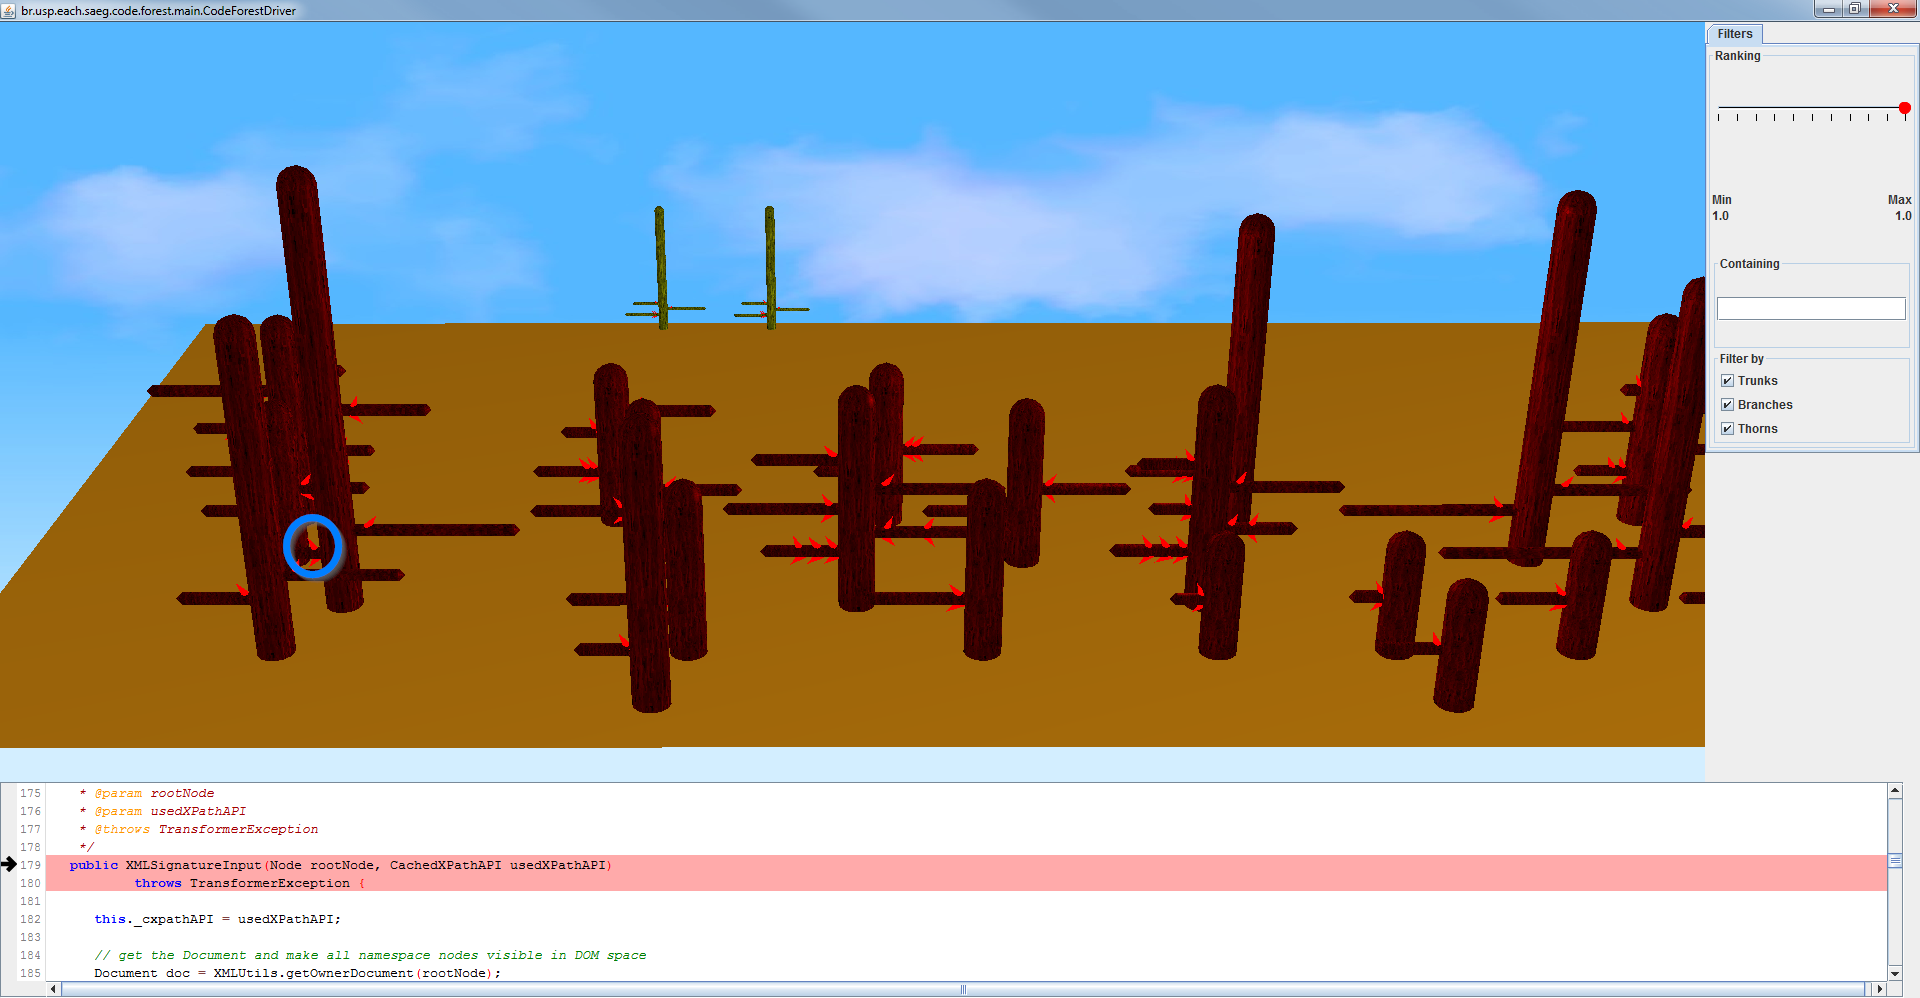
\includegraphics[width=\linewidth]{figures/fig-cf-example-04-alt}
  \caption{View of CodeForest prototype after moving the trimmer to the far right (suspiciousness value equals to 1.0).}
  \label{fig:xml-security-trimmed}
\end{figure*}


A similar behavior happens when developers utilize the filtering tool. By typing
a text in a text box right under the trimmer, the prototype executes a case
insensitive search throughout the whole source code. Every element (cactus,
branch or node) that contains a match is kept on the scene. To keep the forest
metaphor coherent, if a single line of code in a class is a match in a filtering
operation, the minimum cactus is displayed, i.e., the cactus, the branch in
which that line of code was found, and a single thorn, representing the matching
line.
Figure~\ref{fig:xml-security-text-trimmed} exemplifies this situation. The
prototype displays the remaining elements after the term ``XmlSignatureInput''
has been searched.

\begin{figure*}
  \centering
    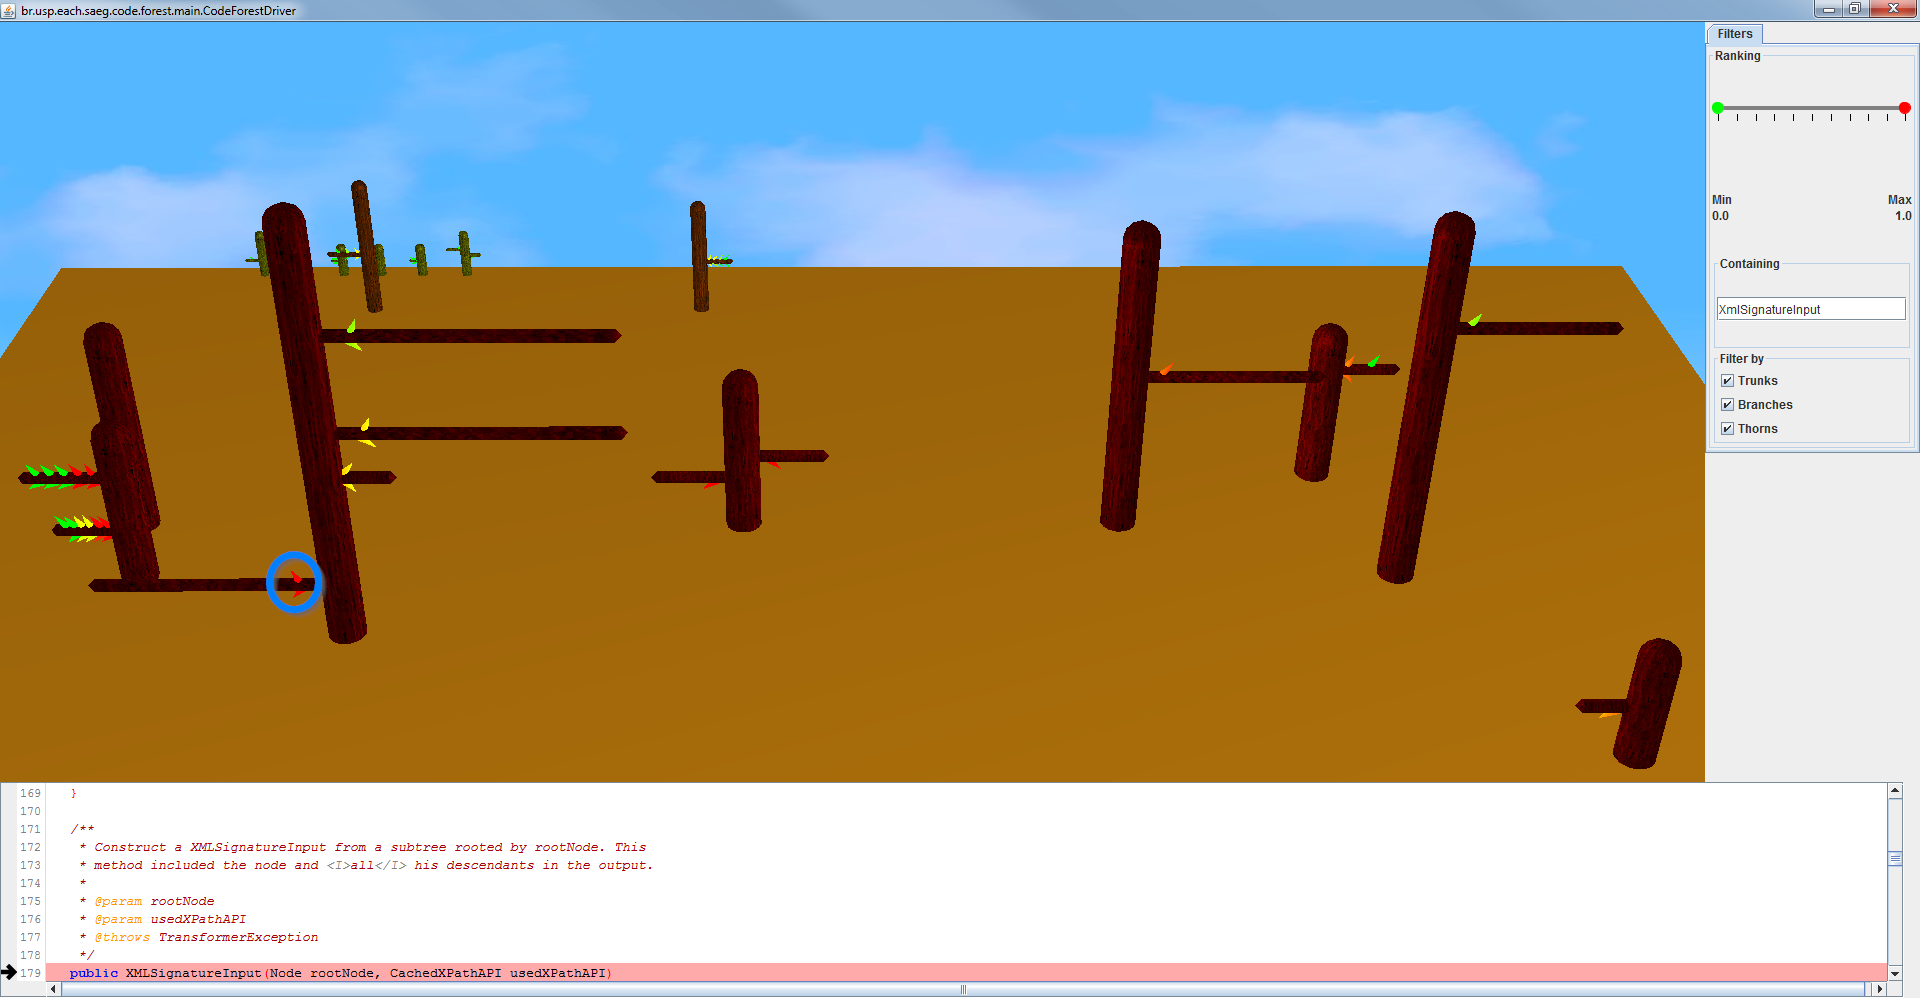
\includegraphics[width=\linewidth]{figures/fig-cf-example-03-alt}
  \caption{View of CodeForest prototype after searching for the term ``XmlSignatureInput''.}
  \label{fig:xml-security-text-trimmed}
\end{figure*}

In Figure~\ref{fig:xml-security-detail}, a suspect thorn is visualized in detail
using the CodeForest prototype. After a zooming operation, its cactus is
enlarged and the thorn to be investigated (highlighted by the blue circle in the
figure) is clicked. After the click, the lines of code associated with the thorn
is presented under the forest (area 2). The color used to paint the code is the
same used to paint the selected thorn.

\begin{figure*}
  \centering
    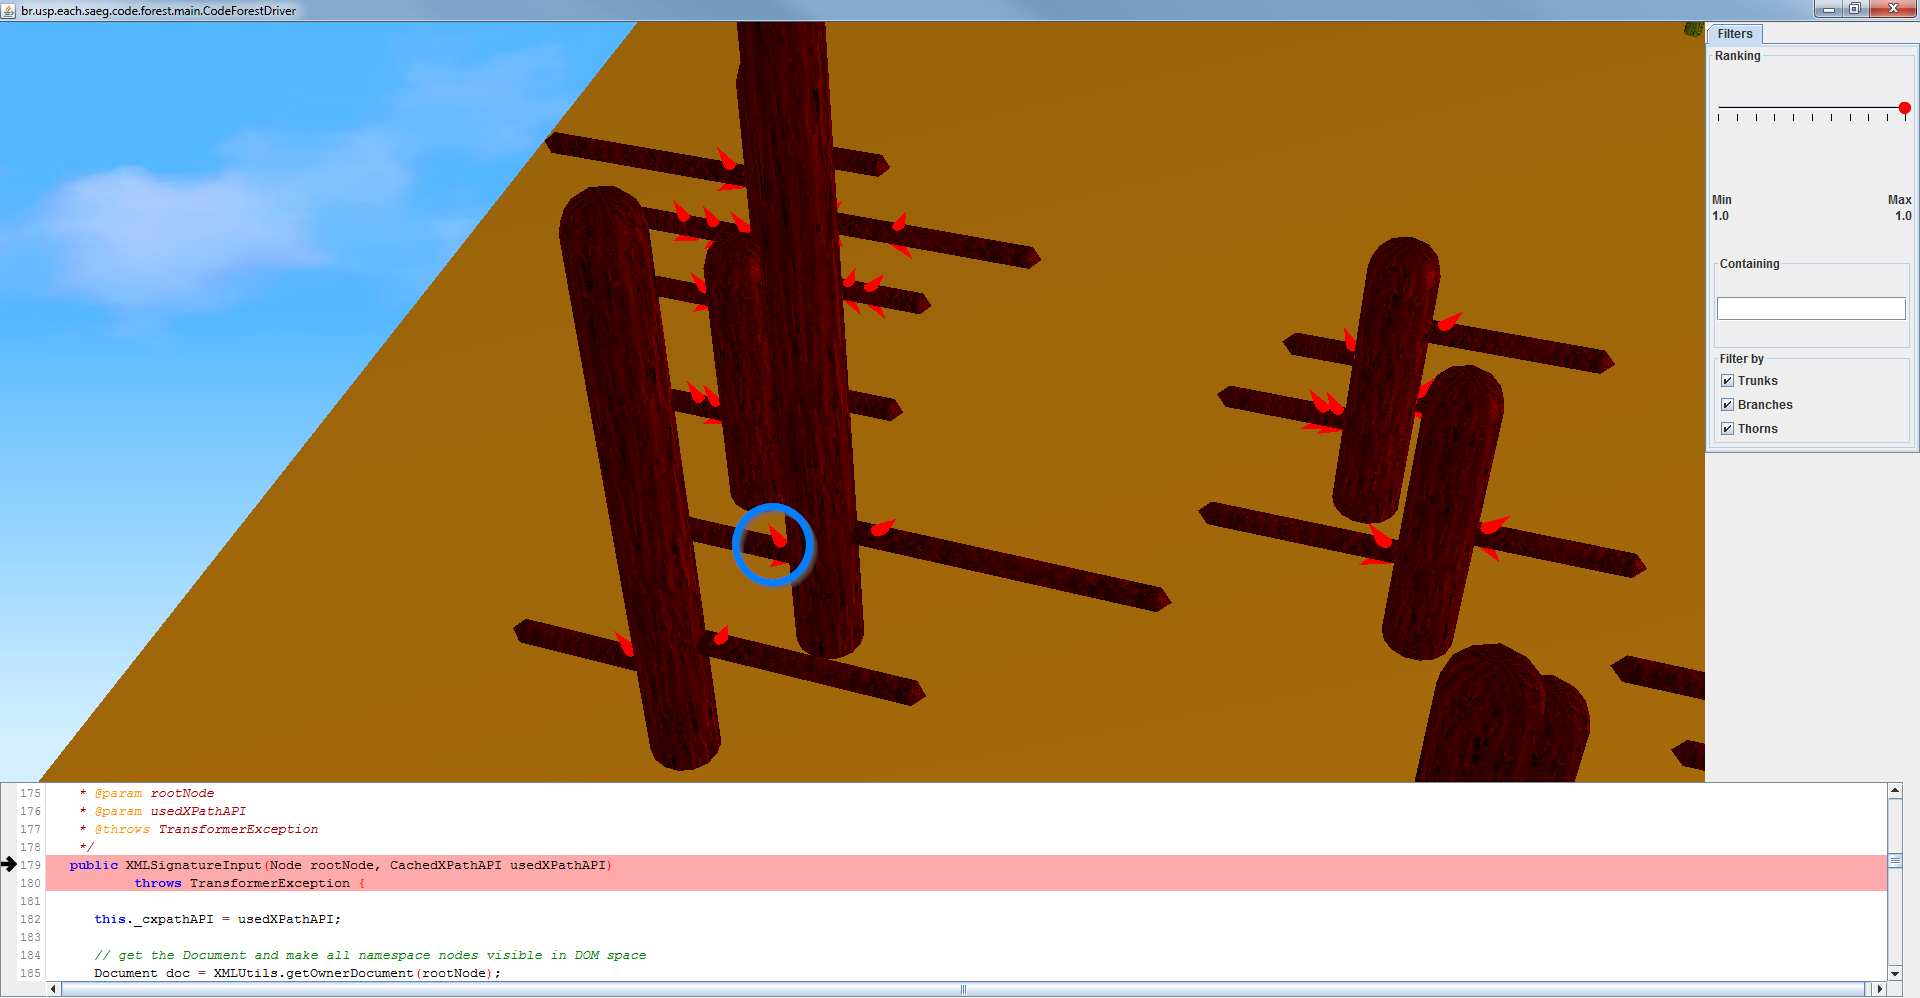
\includegraphics[width=\linewidth]{figures/fig-cf-example-05-alt}
  \caption{Detail of a suspect thorn in CodeForest.}
  \label{fig:xml-security-detail}
\end{figure*}

The trimming and filtering operations play an important role on solving one of
the most common problems found in 3D environments---the occlusion of elements.
With no elements blocking the object of interest, developers are then free to
play with the interface, without making too much effort to select the object of
investigation.

\section{Final Remarks}

In this chapter, we presented the CodeForest metaphor. To the best of our
knowledge, it is the first 3D based metaphor enabling the visualization of the
suspiciousness associated with classes, methods and lines of code (i.e., nodes)
in a hierarchical structure: a forest of cacti.

The CodeForest metaphor allows a large scale vision of a faulty system as well
as mechanisms to debug it. We have present a prototype in which typical 3D
mechanisms (e.g., translation, rotation, and zooming) can be combined with
trimming and filtering operations to localize a fault's site.

Unlike other approaches that utilize the same bothanical tree metaphor for
software visutalization~\cite{kleiberg2001botanical,erra2012towards}, CodeForest
supports developers to  spot suspicious elements in the software structure and
to investigate the piece of code associated with them at the same time. In this
sense, it provides a roadmap from suspicious classes, methods and lines of code
towards the fault's site.

In the next chapter, we present our approach to deploy the Codeforest metaphor
and its debugging operations in an Interactive Development Environment (IDE).